\input{../YKY-preamble.tex}

\usepackage{xeCJK}
\setCJKmainfont[BoldFont=SimHei,ItalicFont=KaiTi]{SimSun}
\usepackage{color}
\usepackage{hyperref}

\usepackage{mathtools}
\usepackage{hyperref}

\title{Symmetric neural networks}
\author{YKY}

\begin{document}
\maketitle

\section{Invariant theory}

Traditional neural network:
\begin{eqnarray}
\boxed{neuron} \quad & y = & \sigmoid \vect{w} \cdot \vect{x} \nonumber \\
\boxed{layer} \quad & y = & \sigmoid W \vect{x} \nonumber \\
\boxed{network} \quad & y = & \sigmoid W \circ \sigmoid W \; .... \; \vect{x} 
\end{eqnarray}

Quadratic neural network:
\begin{eqnarray}
\boxed{neuron} \quad & y = & W \vect{x} \cdot \vect{x} \nonumber \\
\boxed{layer} \quad & y = & W \vect{x} \cdot \vect{x} \nonumber \\
\boxed{network} \quad & y = & W \vect{x} \circ W \vect{x} \; .... \; \vect{x} 
\end{eqnarray}

Traditionally, each neuron $k$ with output $o_k$ is defined as:
\begin{equation}
o_k = \sigmoid ({\text{net}}_k) = \sigmoid \left(\sum _{j=1}^{n} w_{jk} o_j \right) .
\end{equation}

This is replaced by our new neuron:
\begin{equation}
\boxed{\mbox{next layer}} \quad
o_k = {\text{net}}_k = \sum_j \sum_i W_{ij}^k o_i o_j
\quad \boxed{\mbox{current layer}}
\end{equation}
where the 2 summations can be \textbf{interchanged}.

Let $y = F(x)$ denote the (overall) neural network function.  In our case $F(x)$ is a polynomial $\in \mathbb{R}[x]^{\mathfrak{S}_n}$ where $\mathfrak{S}_n$ is the symmetric group of $n$ elements.

This is one quadratic layer with $i > j$ edges deleted (because $x_i x_j = x_j x_i$):
\begin{equation}
\vcenter{\hbox{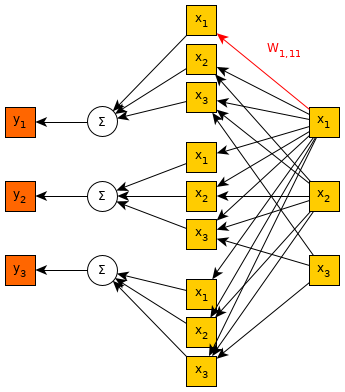
\includegraphics[scale=0.75]{quadratic-NN-2.png}}}
\end{equation}
The link in red is $W_{11}^1$.

This is one network layer complete with quadratic, linear, and constant terms:
\begin{equation}
\vcenter{\hbox{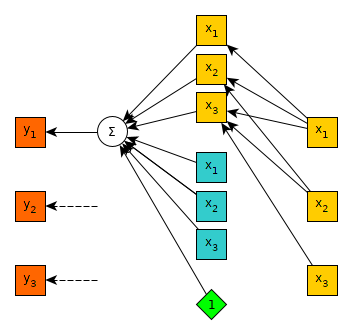
\includegraphics[scale=0.75]{quadratic-NN-3.png}}}
\end{equation}
Notice that this block should be repeated for each output $y_1, ..., y_3$.


\section{General case for $y = W x$}

\begin{equation}
\boxed{\mbox{original}} \quad y_j = \sum_i W_{ij} x_i .
\end{equation}

Equivariance implies:
\begin{eqnarray}
\boxed{\mbox{swapped}} \quad y_j ( \sigma(x_j \; x_k) x) &=& \sigma \cdot y_j = y_k \quad \boxed{\mbox{original}} \\
\sum_{i \neq j,k} W_{ij} x_i + W_{kj} x_j + W_{jj} x_k &=& \sum_{i \neq j,k} W_{ik} x_i + W_{jk} x_j + W_{kk} x_k . \nonumber
\end{eqnarray}

% for $(j \; k) \in \mathfrak{S}_n$.

Comparing coefficients yields:
\begin{eqnarray}
W_{ij} &=& W_{ik} \quad \quad \forall \; j, k, (i \neq j, k) \nonumber \\
W_{kj} &=& W_{jk} \quad \quad \forall \; j, k \nonumber \\
W_{jj} &=& W_{kk} \quad \quad \forall \; j, k .
\end{eqnarray}

In other words, the matrix $W$ is of the form:
\begin{equation}
W = \alpha I + \beta 1 1^T .
\end{equation}

\section{Case for $y_k = W_k x \cdot x$}

The general form of a ``quadratic'' vector function is:
\begin{equation}
y = (A x) \cdot x + B x + C .
\end{equation}

We just focus on the quadratic term $(W x) \cdot x$:
\begin{equation}
\boxed{\mbox{original}} \quad y_k = \sum_j \left[ \sum_{i \le j} W_{ij}^k x_i \right] x_j .
\end{equation}
Note that the matrix $W$ is ``3-dimensional'' and has $N \times N \times N$ entries.

Let $\sigma := (x_k \rightleftharpoons x_h)$, meaning \textbf{transposition} of the two elements.  Equivariance implies:
\begin{equation}
\boxed{\mbox{LHS}} \quad y_k ( \sigma \cdot x) = \sigma \cdot y_k = y_h \quad \boxed{\mbox{RHS}}
% \sum_{j \neq h,k} \sum_{i \neq h,k} W_{ij}^k x_i x_j + W_{hh}^k x_k^2 + W_{kh}^k x_h x_k + W_{hk}^k x_k x_h + W_{kk}^k x_h^2 &=& \sum_{j \neq h,k} \sum_{i \neq h,k} W_{ij}^h x_i x_j + W_{hh}^h x_h^2 + W_{kh}^h x_k x_h + W_{hk}^h x_h x_k + W_{kk}^h x_k^2 \nonumber
\end{equation}

\begin{align}
\boxed{\mbox{LHS}} &= y_k ( \sigma \cdot x ) = \sum_j \left[ \sum_{i \le j} W_{ij}^k  \; \sigma \cdot x_i \right] \sigma \cdot x_j \nonumber \\
&= \sum_j \left[ \sum_{i \le j \atop i \neq h,k} W^k_{ij} x_i + \underbracket[1pt]{W^k_{hj} x_k}_{\text{if } h \le j} + \underbracket[1pt]{W^k_{kj} x_h}_{\text{if } k \le j} \right] \sigma \cdot x_j \quad \quad \boxed{\text{apply } \sigma \cdot x_i} \nonumber \\
% 
&= \sum_{j \neq h,k} \left[ \sum_{i \le j \atop i \neq h,k} W^k_{ij} x_i + \underbracket[1pt]{W^k_{hj} x_k}_{\text{if } h \le j} + \underbracket[1pt]{W^k_{kj} x_h}_{\text{if } k \le j} \right] x_j 
	\quad \quad \quad \boxed{\text{apply } \sigma \cdot x_j} \nonumber \\
	& \quad \quad + \left[ \sum_{i < h \atop i \neq k} W^k_{ih} x_i + W^k_{hh} x_k + \underbracket[1pt]{W^k_{kh} x_h}_{\text{if } k \le h} \right] x_k
	+ \left[ \sum_{i < k \atop i \neq h} W^k_{ik} x_i + \underbracket[1pt]{W^k_{hk} x_k}_{\text{if } h \le k} + W^k_{kk} x_h \right] x_h \nonumber \\
% 
&= \sum_{j \neq h,k} \sum_{i \le j \atop i \neq h,k} W^k_{ij} x_i x_j + {\color{olive}\sum_{j > h} W^k_{hj} x_k x_j} + {\color{cyan}\sum_{j > k} W^k_{kj} x_h x_j} \nonumber \\
& \quad \quad + {\color{blue}\sum_{i < h \atop i \neq k} W^k_{ih} x_i x_k} + W^k_{hh} x_k^2 + {\color{red}  \underbracket[1pt]{W^k_{kh} x_h x_k}_{\text{if } k \le h}} \nonumber \\
& \quad \quad + {\color{red}\sum_{i < k \atop i \neq h} W^k_{ik} x_i x_h} + {\color{blue} \underbracket[1pt]{W^k_{hk} x_k x_h}_{\text{if } h \le k} } + W^k_{kk} x_h^2 \nonumber \\
% 
% ============================================================================================
% 
\boxed{\mbox{RHS}} &= \sum_j \left[ \sum_{i \le j} W_{ij}^h x_i \right] x_j \nonumber \\
% 
&= \sum_j \left[ \sum_{i \le j \atop i \neq h,k} W^h_{ij} x_i + \underbracket[1pt]{W^h_{hj} x_h}_{\text{if } h \le j} + \underbracket[1pt]{W^h_{kj} x_k}_{\text{if } k \le j} \right] x_j \nonumber \\
% 
&= \sum_{j \neq h,k} \left[ \sum_{i \le j \atop i \neq h,k} W^h_{ij} x_i + \underbracket[1pt]{W^h_{hj} x_h}_{\text{if } h \le j} + \underbracket[1pt]{W^h_{kj} x_k}_{\text{if } k \le j} \right] x_j \nonumber \\
& \quad \quad + \left[ \sum_{i < h \atop i \neq k} W^h_{ih} x_i + W^h_{hh} x_h + \underbracket[1pt]{W^h_{kh} x_k}_{\text{if } k \le h} \right] x_h
+ \left[ \sum_{i < k \atop i \neq h} W^h_{ik} x_i + \underbracket[1pt]{W^h_{hk} x_h}_{\text{if } h \le k} + W^h_{kk} x_k \right] x_k \nonumber \\
% 
&= \sum_{j \neq h,k} \sum_{i \le j \atop i \neq h,k} W^h_{ij} x_i x_j + {\color{cyan}\sum_{j > h} W^h_{hj} x_h x_j} + {\color{olive}\sum_{j > k} W^h_{kj} x_k x_j} \nonumber \\
& + {\color{red}\sum_{i < h \atop i \neq k} W^h_{ih} x_i x_h} + W^h_{hh} x_h^2 + {\color{red} \underbracket[1pt]{W^h_{kh} x_k x_h}_{\text{if } k \le h}} \nonumber \\
& + {\color{blue}\sum_{i < k \atop i \neq h} W^h_{ik} x_i x_k} + {\color{blue}\underbracket[1pt]{W^h_{hk} x_h x_k}_ {\text{if } h \le k} } + W^h_{kk} x_k^2
\end{align}

Comparing coefficients yields:
\begin{alignat}{3}
W_{ij}^h &= W_{ij}^k && \forall \; h,k. \; j \neq h,k; \; i \le j; \; i \neq h,k \nonumber \\
{\color{cyan}W_{hj}^h} &= {\color{cyan}W_{kj}^k} && \forall \; h,k. \; j > \max(h,k) \nonumber \\
{\color{olive}W_{kj}^h} &= {\color{olive}W_{hj}^k} && \forall \; h,k. \; j > \max(h,k) \nonumber \\
{\color{cyan}W_{hj}^h} &= {\color{olive}W_{hj}^k} = 0 \quad && \forall \; h,k. \; h < j \le k \nonumber \\
{\color{olive}W_{kj}^h} &= {\color{cyan}W_{kj}^k} = 0 \quad && \forall \; h,k. \; k < j \le h \nonumber \\
{\color{red}W_{ih}^h} &= {\color{red}W_{ik}^k} && \forall \; h,k. \; i \le k; \; i \neq h \nonumber \\
{\color{blue}W_{ik}^h} &= {\color{blue}W_{ih}^k} && \forall \; h,k. \; i \le h; \; i \neq k \nonumber \\
{\color{red}W_{kh}^h} &= {\color{red}W_{kh}^k} && \forall \; h,k. \; k \le h \nonumber \\
{\color{blue}W_{hk}^h} &= {\color{blue}W_{hk}^k} && \forall \; h,k. \; h \le k \nonumber \\
W_{hh}^k &= W_{kk}^h && \forall \; h,k. \nonumber \\
W_{kk}^k &= W_{hh}^h && \forall \; h,k.
\end{alignat}

The following diagram shows the situation of the index $j$ in the {\color{cyan}cyan} and {\color{olive}olive} cases:
\begin{equation}
\vcenter{\hbox{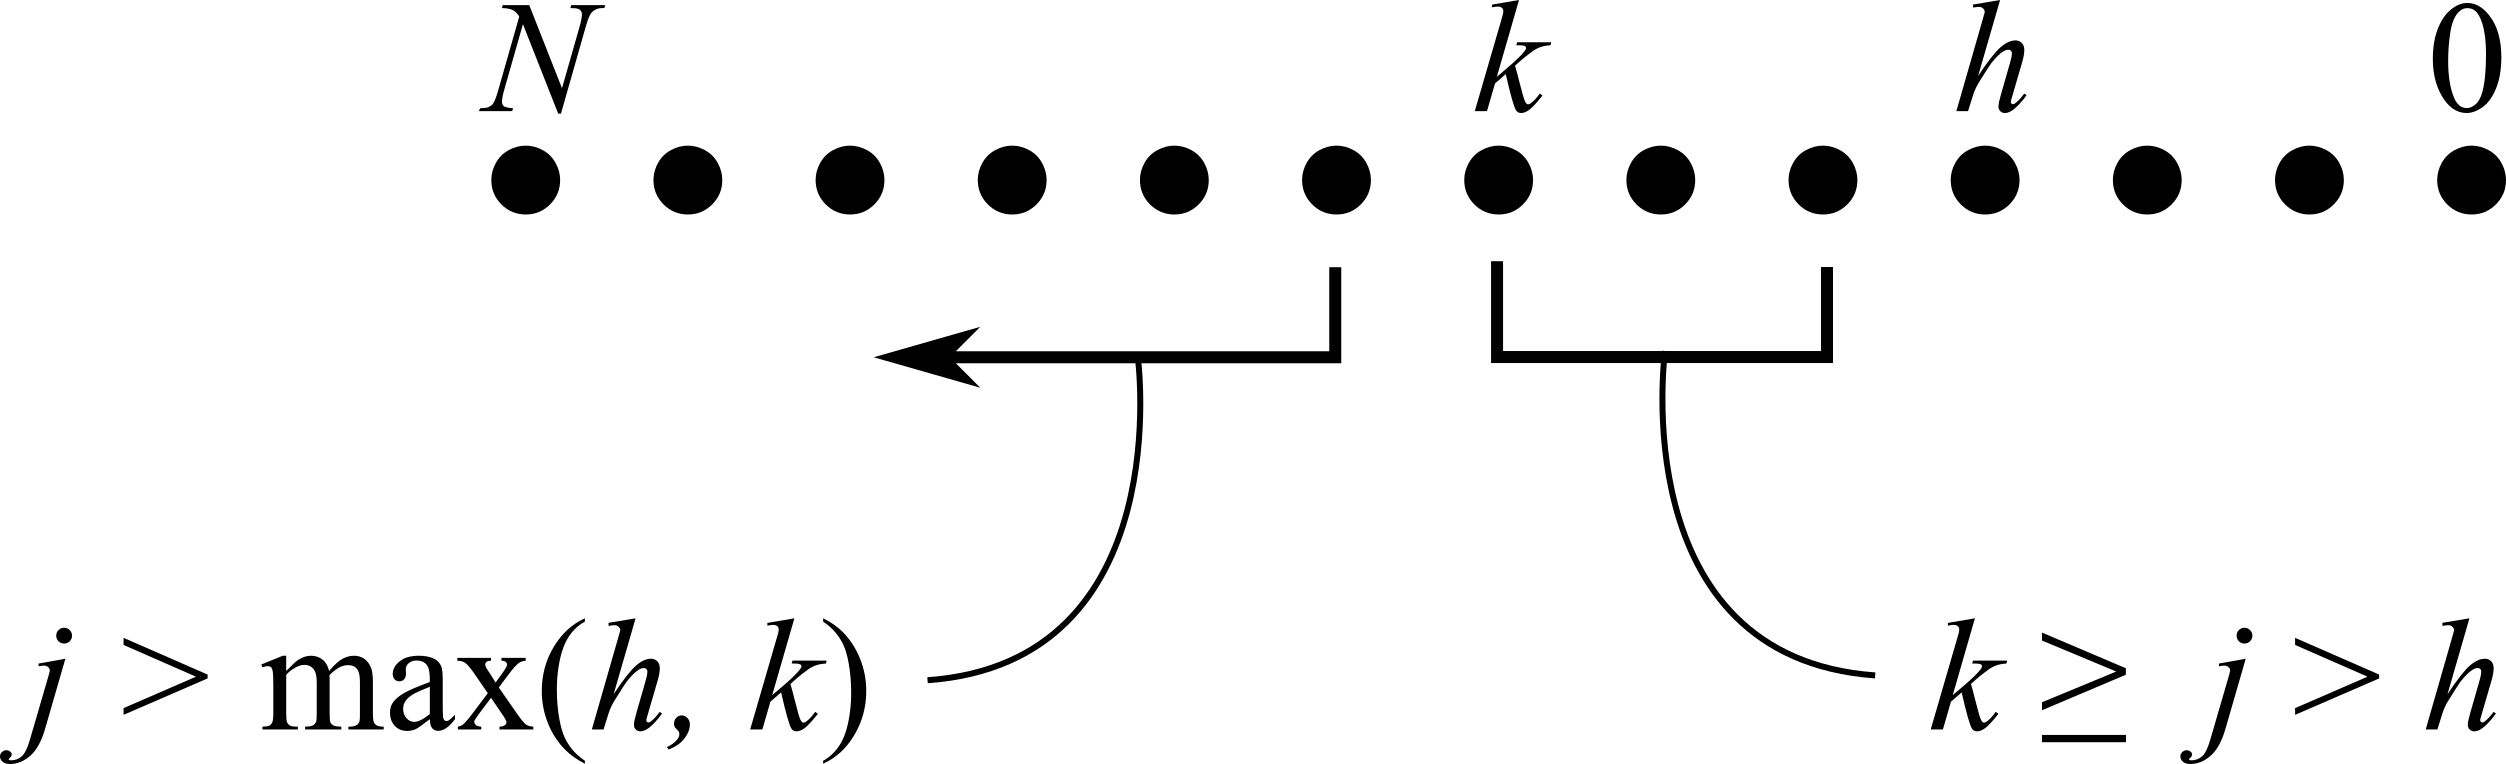
\includegraphics[scale=0.6]{index-j-diagram.png}}}
\end{equation}

How many different colors?
\begin{equation}
\begin{tabular}{l l l l}
$N = 1$ .... & 1 & / 1 & = 100\% \\
$N = 2$ .... & 4 & / 8 & = 50\% \\
$N = 3$ .... & 6 & / 27 & = 22.2\% \\
$N = 4$ .... & 7 & / 64 & = 10.9\% \\
$N = 5$ .... & 8 & / 125 & = 6.4\% \\
$N = 6$ .... & 9 & / 216 & = 4.2\% \\
$N = 7$ .... & 10 & / 343 & = 2.9\% \\
$N = 8$ .... & 11 & / 512 & = 2.1\% \\
$N = 9$ .... & 12 & / 729 & = 1.6\% \\
$N = 10$ .... & 13 & / 1000 & = 1.3\%
\end{tabular}
\end{equation}

There would be $N$ \textbf{blocks} of $N \times N$ matrices.

All diagonals consists of 2 colors, regardless of $N$ (from 2nd and 3rd equations).  This leaves $N (N - 1)$ non-diagonal entries per block.

Non-diagonal entries of different blocks are equal, if the block indices are different from the row and column indices.  Out of $N$ blocks there would be 2 different sets of non-diagonal weights.  (This comes from the 1st equation.)

The last equation causes non-diagonal weights to have a certain symmetry about the diagonal.  

For example, the number of monomials in 3 variables and of degree $\le 8$ is:
\begin{eqnarray}
{10\choose8} + {9\choose7} + {8\choose6} + .... + {4\choose2} + {3\choose1} + {3\choose0} \nonumber \\
= 45 + 36 + 28 + 21 + 15 + 10 + 6 + 3 + 1 = 165
\end{eqnarray}

\section{Programmatic way to find invariant constraints on weights}

Define a scheme to index all the weights in the multi-layer NN: $W_{ij}^{k \ell}$.  Then the entire NN function can be expanded as a polynomial with coefficients from $W$.

For one quadratic layer, there would be a total of $\displaystyle n \left( n^2 - \frac{n (n - 1)}{2} \right) = \frac{n^2 (n + 1)}{2}$ terms.  The coefficients for each term would be composed out of $W_{ij}^{k \ell}$.  Permuting the input would require coefficients of \textbf{like} terms to be equal.  We should try all pairwise permutations of $n$ inputs, of which there are $n (n - 1) / 2$.

On the second layer, the output would be composed of sums and products of polynomials with second-layer weights.  Thus the new coefficients would be \textbf{polynomials} in multi-layer weights.  Invariance or equivariance requires that we compare coefficients of like terms, thus yielding \textbf{equalities with polynomials} on both sides.  Such conditions seems much more complex than the single-layer conditions for equivariance.

This means that the weights would be in an \textbf{algebraic variety} of reduced dimension.  Our objective is to update / learn the weights \textbf{within} this variety.  

\section{Quadratic, multi-layer, unconstrained case}

In the last section we have \textbf{equivariant} layers composed together to form a neural network.  Now we relax the constraints so that the multi-layer network is free to have any weights except that the output must be \textbf{invariant}.


\section{With output space ``folded in half''}

Now suppose the output is only $1/2$ the dimension of the input.  Define a new form of equivariance such that the input permutation would act on the output as ``folded in half''. 

In other words, equivariance is changed to:
\begin{equation}
\boxed{\mbox{swapped}} \quad y_k \cdot \sigma(x_k \; x_h) = y_h \mbox{  or  } y_{h-N/2} \quad \boxed{\mbox{original}} \end{equation}
where $\tau$ is $\sigma$ acting on $y$ as double its length and identifying $y_i = y_{i + N/2}$.

\subsection{Linear case}

Just notice that the dimension of $y$ is halved:
\begin{equation}
\boxed{\mbox{original}} \quad y_j = \sum_i W_{ij} x_i .
\end{equation}

``Folded'' equivariance implies:
\begin{eqnarray}
\boxed{\mbox{swapped}} \quad y_j ( \sigma(x_j \; x_k) x) %\mbox{ or } y_m ( \sigma(x_m \; x_k) x)
&=& \sigma \cdot y_j = y_k \quad \boxed{\mbox{original}} \\
\sum_{i \neq j,k} W_{ij} x_i + W_{kj} x_j + W_{jj} x_k &=& \sum_{i \neq j,k} W_{ik} x_i + W_{jk} x_j + W_{kk} x_k  \nonumber
% \mbox{or } \sum_{i \neq m,k} W_{im} x_i + W_{km} x_m + W_{mm} x_k & & \nonumber
\end{eqnarray}
% where $m = j - N/2$.  This gives rise to 2 sets of equations.
with the restriction $j \in \{ 1,..., N/2 \}$, and $k \in \{ 1,..., N \}$.

The constraints obtained are same as before, except that index ranges are different:
\begin{eqnarray}
W_{ij} &=& W_{ik} \quad \quad \forall \;  j, k, (i \neq j, k) \nonumber \\
W_{kj} &=& W_{jk} \quad \quad \forall \;  j, k \nonumber \\
W_{jj} &=& W_{kk} \quad \quad \forall \;  j, k \nonumber
%\hline \nonumber\\
%W_{ij} &=& W_{ik} \quad \quad \forall \;  j > N/2, k \le N/2, (i \neq j, k) \nonumber \\
%W_{kj} &=& W_{jk} \quad \quad \forall \;  j > N/2, k \le N/2 \nonumber \\
%W_{jj} &=& W_{kk} \quad \quad \forall \;  j > N/2, k \le N/2 \nonumber\\
%\hline \nonumber\\
%W_{ij} &=& W_{ik} \quad \quad \forall \;  j \le N/2, k > N/2, (i \neq j, k) \nonumber \\
%W_{kj} &=& W_{jk} \quad \quad \forall \;  j \le N/2, k > N/2 \nonumber \\
%W_{jj} &=& W_{kk} \quad \quad \forall \;  j \le N/2, k > N/2 \nonumber\\
%\hline \nonumber\\
%W_{ij} &=& W_{ik} \quad \quad \forall \;  j > N/2, k > N/2, (i \neq j, k) \nonumber \\
%W_{kj} &=& W_{jk} \quad \quad \forall \;  j > N/2, k > N/2 \nonumber \\
%W_{jj} &=& W_{kk} \quad \quad \forall \;  j > N/2, k > N/2
\end{eqnarray}

These constraints give rise to a matrix of this form (for the $6 \times 3$ case, numbers represent different colors):
\begin{equation}
\begin{tabular}{c c c c c c c}
5 & 1 & 1 & 2 & 3 & 4 & \\
1 & 5 & 1 & 2 & 3 & 4 & \\
1 & 1 & 5 & 2 & 3 & 4 & .
\end{tabular} 
\end{equation}This pattern is obtained from my Python code.

NOTE:  The above pattern is verified to be NOT equivariant, there is a bug in the equivariant condition.

\subsection{Quadratic case}

\section{Learning algorithm}

作者:zighouse

链接:\url{https://www.zhihu.com/question/327765164/answer/704606353}

来源:知乎

著作权归作者所有。商业转载请联系作者获得授权,非商业转载请注明出处。

神经网络是对一类内部结构固定的非线性函数的俗称,这类函数是输出关于输入以及隐含内部状态的函数,输出与输入呈现非线性特性。当一份输出只与一份输入有关时,常用卷积神经网络来实现。当一份输出与一个相继表达的输入序列相关时,可以用回归神经网络来实现。一般地,神经网络可以技术性地分解成神经元的复合,这里的神经元是在这个神经网络中的一种最基本的非线性函数的俗称,管理着属于它的内部状态,并基于这些内部状态在神经网络中负责着分配到它的非线性处理。每多一重基本非线性函数的复合,则多一层神经元。如果在某一重复合中出现了两类或者更多类基本非线性函数项的合并,则出现了分支。

神经网络的权值是分解到具体神经元管理的一种内部状态。用反向传播方法来更新神经网络的权值是基于这样一个基本的假设:在一个确定的输入(或者输入序列)并产生当前输出的这个点(权值构成的线性空间中的点)上,输出在这个点上是连续的。即权值点的连续微小变化会导致输出点相应的连续微小变化。这样,当我们希望调节当前权值以使此输出向特定点靠拢时,就得出了基于权值空间中错误/误差/惩罚的梯度的反向传播算法。

如果想在某个神经网络中的两个权值间建立一种约束关系,这两个权值自然就不再相互独立,可以通过考查整个权值构成的线性空间,秩会变小。约束条件只要不改变连续假设,仍然可以求出带约束条件下的梯度。如果改变了连续假设,则意味着非线性分解不恰当,需要重新分解神经网络的基本结构。

\subsection{Classic back-prop with quadratic neurons}

Traditional neural network:
\begin{eqnarray}
\boxed{neuron} \quad & y = & \sigmoid \vect{w} \cdot \vect{x} \nonumber \\
\boxed{layer} \quad & y = & \sigmoid W \vect{x} \nonumber \\
\boxed{network} \quad & y = & \sigmoid W \circ \sigmoid W \; .... \; \vect{x} 
\end{eqnarray}

Quadratic neural network:
\begin{eqnarray}
\boxed{neuron} \quad & y = & W \vect{x} \cdot \vect{x} \nonumber \\
\boxed{layer} \quad & y = & W \vect{x} \cdot \vect{x} \nonumber \\
\boxed{network} \quad & y = & W \vect{x} \circ W \vect{x} \; .... \; \vect{x} 
\end{eqnarray}

Traditionally, each neuron $k$ with output $o_k$ is defined as:
\begin{equation}
o_k = \sigmoid ({\text{net}}_k) = \sigmoid \left(\sum _{j=1}^{n} w_{jk} o_j \right) .
\end{equation}

This is replaced by our new neuron:
\begin{equation}
\boxed{\mbox{next layer}} \quad
o_k = {\text{net}}_k = \sum_j \sum_i W_{ij}^k o_i o_j
\quad \boxed{\mbox{current layer}}
\end{equation}
where the 2 summations can be \textbf{interchanged}.

What follows is just a re-working of traditional back-propagation.

Using the chain rule:
\begin{equation}
\frac{\partial E}{\partial W_{ij}^k}
= \frac{\partial E}{\partial o_k} \frac{\partial o_k}{\partial W_{ij}^k}
\end{equation}

For the RHS's second factor, only one term in the sum depends on $W_{ij}^k$, so:
\begin{equation}
	\label{eqn:do-k-dW}
\frac{\partial o_k}{\partial W_{ij}^k}
= \frac{\partial }{\partial W_{ij}^k} \left( \sum_{i'} \sum_{j'} W_{i' j'}^k o_{i'} o_{j'} \right)
= \frac{\partial }{\partial W_{ij}^k} W_{ij}^k o_i o_j = o_i o_j .
\end{equation}

If $k$ is an inner neuron, let $L = \{ u, v, \dots , w \}$ be the \textbf{next layer} of neurons receiving input from neuron $k$.  Consider $E$ as a function with the inputs being all neurons in $L$:
\begin{eqnarray}
\frac{\partial E(o_k)}{\partial o_k}
&=& \frac{\partial E(o_u, o_v, \dots, o_w)}{\partial o_k} \nonumber \\
\boxed{\mbox{next layer}} \quad
	o_{\ell} &=& \sum_j \sum_i W_{ij}^{\ell} o_i o_j
\quad \boxed{\mbox{current layer}}
\end{eqnarray}
and take the total derivative with respect to $o_k$.  A \textbf{recursive} expression for the derivative is obtained:
\begin{equation}
	\label{eqn:dE-do-k}
\frac{\partial E}{\partial o_k}
= \sum_{\ell \in L} \left( \frac{\partial E}{\partial o_{\ell}} \frac{\partial o_{\ell}}{\partial o_k} \right)
= \sum_{\ell \in L} \left( \frac{\partial E}{\partial o_{\ell}} \sum_j W_{kj}^{\ell} o_j \right)
\end{equation}

Substituting, we obtain:
\begin{eqnarray}
\frac{\partial E}{\partial W_{ij}^k}
&=& \frac{\partial E}{\partial o_k} \frac{\partial o_k}{\partial W_{ij}^k}
= \frac{\partial E}{\partial o_k} o_i o_j := \delta_k o_i o_j \nonumber \\ 
\delta_k &=& \sum_{\ell \in L} \left( \delta_{\ell} \sum_j W_{kj}^{\ell} o_j \right)
\end{eqnarray}

Our algorithm can be compared the classic back-prop algorithm:
\begin{eqnarray}
\frac{\partial E}{\partial W_{i j}} &=& \delta_j o_i \nonumber \\
\delta_j &=& \frac{\partial E}{\partial o_j} \frac{\partial o_j}{\partial \mathrm{net}_j} =
	\begin{cases}
	\displaystyle
	\frac{\partial L}{\partial \sigmoid(o_j)} \frac{\partial \sigmoid(o_j)}{\partial o_j} & \text{if $j$ = output neuron} \\
	\displaystyle
	\sum_l W_{j l} \delta_l \frac{\partial \sigmoid(o_j)}{\partial o_j} &  \text{if $j$ = inner neuron} 
	\end{cases}
\end{eqnarray}

\subsection{Shared weights}

For our purpose, it is good to know that all the weight-sharing occurs \textbf{within} each layer, never across layers.

The coefficient of $x_i x_j$ is $W_{i j}$, for the $y_k$ component.  For each weight $W_{ij}^k$ we need to calculate the gradient $\displaystyle \frac{\partial E}{\partial W_{ij}^k}$, but the weights are in equivalence classes.

Say if the following 2 weights are shared:
\begin{equation}
W_0 := W_{i j} \equiv W_{i' j'}
\end{equation}
Then the network:
\begin{equation}
y = \sum \sum W_{ij} x_i x_j
\end{equation}
would contain the shared components:
\begin{equation}
W_0 ( x_i x_j + x_{i'} x_{j'} ) + \mbox{other terms ...}
\end{equation}

\subsubsection{Equality constraints}

For simple \textbf{equality} of weights, the weights should be collected together.  (\ref{eqn:do-k-dW}) should simply be $\sum o_i o_j$ for the equivated weights.

\subsubsection{Additive constraints}

The most tricky part is the ``additive'' constraint:
\begin{equation}
W_{hk}^h + W_{kh}^h = W_{hk}^k + W_{kh}^k \quad \forall \; h,k .
\end{equation}

This is just like having 4 ``not quite independent'' variables $x, y, u, v$ satisfying:
\begin{equation}
x + y = u + v
\end{equation}
and asking what is
\begin{equation}
\frac{\partial (x + y)}{\partial x} \mbox{ ?}
\end{equation}
And the solution is to make one of the variables \textbf{depend} on the other 3.

For each layer, iterate over every neuron representative, which has a collection of coefficients.

We need to consider equations (\ref{eqn:do-k-dW}) and (\ref{eqn:dE-do-k}), but (\ref{eqn:dE-do-k}) is unaffected by weight-sharing.

In (\ref{eqn:do-k-dW}), for each equivalence class, 

\end{document}